\documentclass{article}
\usepackage{graphicx} % Required for inserting images
\usepackage{geometry}
\newgeometry{vmargin={15mm}, hmargin={12mm,17mm}} 
\title{SEMSANS at the cold neutron source in Delft}
\author{Thom van der Woude}
\date{June 2024}
%Universal prelude for everything sciency, mathy, and what have you
%Make semantic macros, not syntactic macros!
%maths stuff
\usepackage[stretch=10]{microtype}
\usepackage{todonotes}
\usepackage{amsfonts,amsmath, amssymb,amsthm,steinmetz}
\usepackage[utf8]{inputenc}
%nice tables
\usepackage{booktabs}
\usepackage{multicol}
\usepackage{chemfig}
\usepackage{lmodern}
\usepackage{enumitem}
%units for doing a science. allowlitunits means things like 20\milli\meter in math mode without \SI{}{}
\usepackage{siunitx}
%time, you always need time
\usepackage{datetime}
%semi-nice karnaugh maps which can be defined using minterms, maxterms etc.
\usepackage{karnaugh-map}
\newtheorem{theorem}{Theorem}
\usepackage{marginnote}
\usepackage{tikz}
\usepackage{subcaption}
\usepackage[normalem]{ulem}
\usepackage{graphicx} 
\usetikzlibrary{quotes,angles}
%\dv <3
\usepackage{physics}
%bra-ket notation for quantum stuff
\usepackage{braket}
%for surface and volume integrals
\usepackage{esint}
\usepackage{enumitem}
%Specific hackery/macros to save time/make latex more semantic less syntactic
\DeclareMathOperator{\sinc}{sinc}
\newcommand{\conj}[1]{\,\overline{\!{#1}}}
\newcommand{\phasor}[1]{\,\widetilde{\!{#1}}}
\newcommand{\risingfac}[1]{%
	^{\overline{#1}}%
}
%for sets generating groups
\newcommand{\gen}[1]{%
	\langle #1\rangle
}
\newcommand{\fallingfac}[1]{%
	^{\underline{#1}}%
}
%Theorem style for "[Name of famous mathematician]'s Theorem" type of theorems, of which there are a surprising number.
\theoremstyle{named}
\newtheoremstyle{named}{}{}{\itshape}{}{\bfseries}{.}{.5em}{\thmnote{#3's }#1}
\newcommand{\bitvector}[2]{
	\underline{#1} = (#1_{#2-1},#1_{#2-2},...,#1_0)
}
\newcommand{\code}[1]{
	\texttt{#1}
}
\newcommand{\mean}[1]{
	\langle #1 \rangle
}
\usepackage[leqno]{mathtools}
\usepackage{chngcntr}
\counterwithin{equation}{section}
\usepackage[roman, thin, thinp, thinc]{esdiff}

\usepackage{bm}
\usepackage{marginnote}
\usepackage{epigraph}
\usepackage{hyperref}
\usepackage[
backend=biber,
%sorting=ynt
]{biblatex}

\addbibresource{references.bib}
\newcommand{\targetrange}{$10 \unit{\nano\meter}$ to $5 \unit{\micro\meter}$ }
\begin{document}

\maketitle

\section{Introduction}
In the food industry, there is the need to analyse the structure of materials at length scales ranging from nanometres to millimetres. To do this, different methods exist such as scattering techniques, microscopy and analysis based on macroscopic properties. What is unique about scattering techniques however is that they can probe the bulk of the sample at these length scales \cite{bouwman2021}.

% I need to add a better bridge between these two sections, they are both good but lack coupling.

\subsection{Small-angle scattering}

Different scattering techniques exist based on X-rays and neutrons. Generally speaking, because these are reciprocal space methods, larger length-scales correspond to smaller scattering angles and vice versa. This is the motivation behind small-angle scattering methods like Small Angle X-ray Scattering (SAXS) and Small Angle Neutron Scattering (SANS) which are used to analyse materials at length scales from $1 \unit{\nano\meter}$ to a few $100 \unit{\nano\meter}$, which are significantly larger than for instance crystal lattice constants of a few $\unit{Å}$ that can be determined using techniques like X-ray diffraction. Past the upper limit of a few $100 \unit{\nano\meter}$ such small-angle techniques become infeasible for realistic beam sizes and samples, as the deflection of particles in a beam is too slight to learn something about the sample.

For neutrons, spin polarization can be used to label trajectories across the beam, a technique called neutron spin echo \cite{mezei1972}. This principle has been applied in the SANS-derivative techniques SESANS \cite{rekveldt1996} and SEMSANS \cite{bouwman2009}\cite{bouwman2011} to make smaller angles and correspondingly the larger length scales up to about $10 \unit{\micro\meter}$ accessible using polarized neutrons. Formulated differently, these techniques can be seen to measure a type of real-space density correlation function $G(\delta)$ \cite{krouglov2003}\cite{andersson2008} as will also be discussed in Chapter \ref{c2:theory}.

\subsection{SEMSANS at the Reactor Institute Delft}


SEMSANS instruments have previously been realized at the Hoger Onderwijs Reactor (HOR) at the Reactor Institute Delft (RID) using a thermal neutron source. As part of the OYSTER project (Optimized Yield for Science, Technology, and Education of Radiation), a cold neutron source operating at $T=20 \unit{\kelvin}$ has been installed and additional improvements have been made to achieve an expected hundredfold improvement in measurement quality or time.

In this report, the possibility for realizing a SEMSANS instrument at the new cold source at HOR will be explored through a combination of mathematical analysis, constrained optimization and Monte Carlo simulations using raytracing software package McStas \cite{willendrup2020}. An existing McStas simulation model \cite{bouwman2021b} is taken as a starting point and extended to include various design options such as precession devices different from foil flippers. 
The goal is to bridge the gap between accessible length ranges of SANS and SEMSANS \cite{bouwman2021} and see if it is possible to access characteristic lengths from \targetrange in a single instrument by exploiting the advantage of greater wavelengths. This as an alternative to combining SANS and SEMSANS devices into one as has been proposed before \cite{bouwman2011}\cite{kusmin2017}. An application that would benefit from such an instrument is the study of colloids such as casein micelles in (fat free) milk and derivatives like yoghurt and curd. The characteristic length scales of all of these would be accessible at an instrument with this target range, facilitating a better understanding of processes like milk turning into yoghurt. 

\newpage 
\section{Theory}
\label{c2:theory}
In this chapter, a review is given of relevant theory related to SEMSANS and the interpretation of measurements. First, the basic principles of SEMSANS as a neutron spin echo technique are explained and the way the beam is modulated is derived. Next, the interaction of samples with the modulated beam is discussed and the concept of spin-echo length $\delta$ is introduced.

% I like 'Beam modulation through Larmor precession' as a phrase
\subsection{Polarized neutrons and Larmor precession}
\label{c2.1}
Neutrons are spin $s=\frac{1}{2}$ particles, meaning that their spin can be described as a superposition of spin states $\{\ket{\uparrow}, \ket{\downarrow}\}$ for some chosen axis or equivalently using a spin angular momentum vector $\vec{S}$, the direction of $\vec{S}$ being the spin polarization $\vec{P}$.
When a neutron passes through a uniform $\vec{B}$-field, $\vec{P}$ will precess by a certain angle $\phi$ over time. The frequency at which this occurs is given by
$$\omega = \gamma |B_\perp|$$
with $B_\perp$ the magnetic field strength perpendicular to the plane $\vec{P}$ is in and $\gamma$ the neutron gyromagnetic ratio. 

In addition to spin, a neutron has a wavelength $\lambda$ corresponding to a speed $v = \frac{h}{m\lambda}$, $m$ being the neutron mass. This means that it will pass through a uniform (perpendicular) field $B$ of length $L$ in time $t = \frac{Lm\lambda}{h}$. From this it can be seen that the total precession will be 
\begin{equation}
	\phi = \frac{\gamma B L m\lambda}{h} = c\lambda B L \label{eq:larmor-prec}
\end{equation}
with $c = \frac{\gamma m}{h}$ being the Larmor constant \cite{bouwman2021b}.   
\subsection{Modulating a neutron beam using precession}
\label{c2.2}
Using the concepts of polarized neutrons and Larmor precession, the basic concept of a SEMSANS instrument can be described, deferring a detailed discussion of the source and monochromator for now. The instrument takes a neutron beamline as a source, meaning that with the choice of axes used in this research neutrons can be assumed to move in the $z$-direction with a slight divergence in the $xy$ plane. A polarizer is used to polarize the beam in the $+x$ direction. Next, the beam passes through two precession devices at distance $L_1, L_2$ from the detector that give neutrons at wavelength $\lambda$ in the beam a $y$-dependent precession angle
\begin{equation}
	\phi = 2\pi\alpha\lambda y \label{eq:precession-freq}
\end{equation}
Such a $y$-dependent $\phi$ is in practice created using magnetic fields at an angle $\theta_0$ with the beam axis $z$. Different precession devices exist which can create such fields as will be analysed and discussed in Section [PLACEHOLDER].

Finally, the modulation is created by applying an analyser to the beam afterwards \cite{mezei1972}. This again polarizes the beam in either the $+x$ or the $-x$ direction depending on the analyzer setting. Assuming a perfectly monochromatic source with $\lambda = \lambda_0$ for all neutrons and ignoring the effect of the sample for now, this creates an intensity modulation pattern on the position-sensitive detector at frequency $f_0 = \alpha\lambda_0$ of the form
\begin{equation}
	I_{b,s}(y) = I_{0, b,s} \pm A_{b,s}\cos(2\pi f_0y) \label{eq:mono-modulation}
\end{equation}
where $I_{b,s}, A_{b,s}$ are experimentally observed quantities in the base case of an empty instrument ($b$) and an instrument with a sample ($s$) and the sign of the modulation depending on the $\pm x$ analyser setting \cite{parnell2023}. 
\subsection{Spin-echo length $\delta$ and measurement interpretation}
\label{c2.3}
When adding a sample to the instrument after the analyser at distance $L_s$ from the detector, a length scale known as the spin-echo length $\delta$ is accessed \cite{bouwman2011}, given by 
\begin{equation}
	\delta = \lambda_0^2L_s\alpha \label{eq:delta}
\end{equation}
This is the same spin-echo length as used in the analysis and interpretation of SESANS \cite{rekveldt1996}\cite{krouglov2003}\cite{andersson2008}. Whereas in SESANS a decrease in overall beam polarization is used, SEMSANS considers the reduction of intensity modulation amplitude or equivalently visibility upon adding a sample, which can be shown to be related to $\delta$ through the formula \cite{parnell2023}
\begin{equation}
	\frac{A_s(\delta)}{A_b(\delta)} = P(\delta) = e^{G(\delta) - \tau} \label{eq:sample-pol-reduction}
\end{equation}
with $\tau = \sigma t$ being the scattering power, which corresponds to the average number of scattering events for a neutron traversing the sample. $G(\delta)$ is the SESANS correlation function given by
$$G(\delta) = \frac{1}{k_0^2}\int dQ_xdQ_y \dfrac{d\sigma(\vec{Q})}{d\Omega}cos(Q_y \delta)$$
This is the 1D expression for $G(\delta)$ compatible with anisotropic samples and also matching the 1D detector that will be described in the next chapter. In the case of isotropic samples, radial integration is possible without loss of information and $G(\delta)$ can be stated using a Hankel transform instead of a cosine transform \cite{andersson2008}.

\subsection{Mono-disperse reference sample and its $G(\delta)$}
\label{c2.4}
Expressions for $\tau$ and $G(\delta)$ exist and can be derived for many different sample geometries \cite{andersson2008}. In the context of analysing colloidal systems, a simple commonly used model is a dilute mono-disperse solution of solid spheres \cite{tromp2007}. Although poly-disperse models such as log-normal distributions of spheres appear to better match real samples \cite{heijkamp2011}, a mono-disperse sample is used as a reference in this work as it is also implemented in McStas in the form of the \texttt{SANS\_spheres2} component (see \cite{parnell2024} for a validation of this sample in the context of SESANS) in addition to being a simpler model for samples of various characteristic lengths. 

Such a mono-disperse sample is characterized by sphere radius $R$, scattering length density contrast $\Delta\rho$, volume fraction $\phi$ and lastly a sample thickness $t$. The scattering power $\tau$ for such a sample is given by

\begin{equation}
	\tau = \frac{3}{2}\phi (1 - \phi) (\Delta\rho)^2\lambda_0^2tR \label{eq:sample-tau}
\end{equation}
Using $\xi = \frac{\delta}{R}$, it can be derived that for $0\leq \xi \leq 2$, $G(\delta) = \tau G_0(\delta)$ with 
\begin{equation}
	G_0(\delta) = \left[1 - \left(\frac{\xi}{2}\right)^2\right]^{1/2}\left(1 + \frac{1}{8}\xi^2\right) + \frac{1}{2}\xi^2\left[1 - \left(\frac{\xi}{4}\right)^2\right]\ln \left[\frac{\xi}{2 + (4 - \xi^2)^{1/2}}\right] \label{eq:sample-G0}
\end{equation}
Outside of this range, $G_0(\xi) = 0$ \cite{krouglov2003}. Figure \ref{fig:analytical-G0} shows $G_0(\delta)$ for different values of $R$. 

\begin{figure}
	\centering
	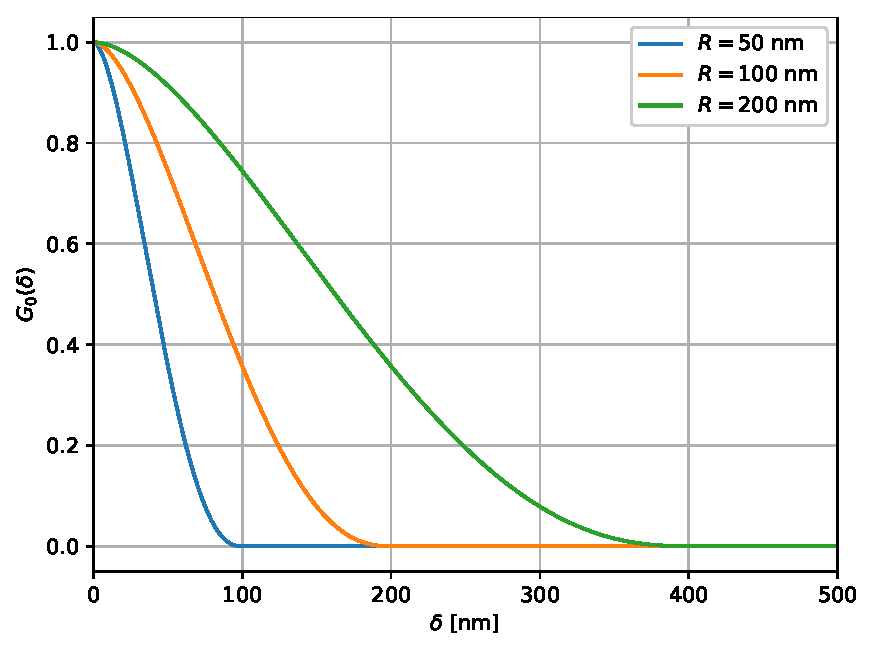
\includegraphics[width=0.5\linewidth]{analytical-G0}
	\caption{TODO}
	\label{fig:analytical-G0}
\end{figure}
\newpage

\begin{figure*}
	\centering
	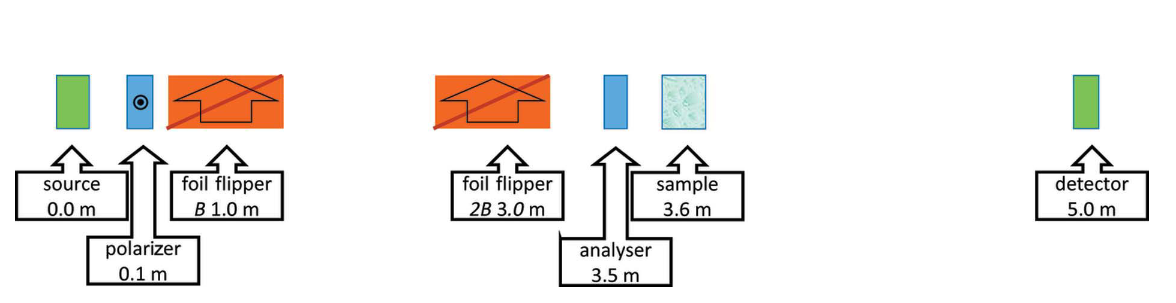
\includegraphics[width=\linewidth]{config-placeholder}
	\caption{PLACEHOLDER IMAGE, TO BE REPLACED}
	\label{fig:instrument-config}
\end{figure*}
\section{Instrument analysis for a cold source}
In this chapter, the used SEMSANS instrument model is introduced and analysed. The cold neutron source and the applicable monochromators for different $\lambda_0$ ranges will be described and three different precession device options and their properties will be described. Additionally, the effect of a spread in wavelength $\lambda$ is described in terms of the observed modulation pattern as well as what is effectively measured. This is to account especially for the greater wavelength spread $\Delta\lambda/\lambda_0$ as encountered at higher $\lambda_0$ operating points accessible at a cold source, requiring the use of a velocity selector monochromator. In the last section the list of instrument design variants considered in this research is introduced. These will be analysed and simulated in Chapter \ref{c4:constraints} and Chapter \ref{c6:monte-carlo} respectively. 

\subsection{Instrument configuration}
The general configuration of the family of SEMSANS instruments considered in this work is illustrated in Figure \ref{fig:instrument-config}. It is derivative of an existing study simulating a SEMSANS instrument using foil-flippers and the corresponding McStas instrument \texttt{SEMSANS\_Delft} \cite{bouwman2021b}. Neutrons enter the instrument from a beamline, after which they pass through a monochromator set to select neutrons with a wavelength around $\lambda_0$, with  $\Delta\lambda/\lambda_0$ depending on the choice of monochromator as described below. Next, they pass through a polarizer and two precession devices at locations $L_1, L_2$ respectively. As described in Chapter \ref{c2:theory}, a modulated neutron intensity pattern appears after the analyser, which scatters of the sample at distance $L_s$ from the position-sensitive detector at the end, causing different degrees of loss of visibility of the modulation pattern depending on the sample structure. 

\subsection{Source and monochromators}
The cold source beamline is assumed to have a spectrum corresponding to a Maxwell-Boltzmann distribution at $T = 20 \unit{\kelvin}$ given by 
\begin{equation}
	f_\lambda(\lambda) = \sqrt{\frac{2}{\pi}}\left(\frac{1}{mk_BT}\right)^{\frac{3}{2}}\frac{h^3}{\lambda^4}e^{-\frac{h^2}{2k_BTm\lambda^2}} \label{eq:cold-source-spectrum}
\end{equation}
This distribution is shown in Figure \ref{fig:source-spectrum}, with the thermal distribution at $T=290 \unit{\kelvin}$ also shown for reference. The peak for $T=20 \unit{\kelvin}$ corresponds to $E = k_bT = 1.724 \unit{\milli\electronvolt}$ as opposed to $E = 24.990 \unit{\milli\electronvolt}$ for room-temperature neutrons. 

A monochromator is used to select a narrow band of wavelengths around a central wavelength $\lambda_0$. In a practical instrument, a pyroletic graphite (PG) crystal monochromator can be used to do this up to roughly $\lambda_0 \approx 4.5 $Å. For greater wavelengths, a helical velocity selector (VS)\cite{szewc2010} can be used to select neutrons travelling at the right velocity. This is a mechanical device rotating at a great speed, and a lower practical limit of $\lambda_0 \approx 7$Å is used as lower $\lambda_0$ would require a too great RPM. Both types of monochromator are characterized by $\Delta\lambda/\lambda_0$, the ratio of the full-width-half-maximum (FWHM) of wavelengths $\Delta\lambda$ passed through and $\lambda_0$. In PG crystals, this is a function of the mosaicity of the crystal \cite{shapiro1972} and for VS monochromators it depends on the ratio of the angular aperture of slits and the pitch angle \cite{szewc2010}. This ratio is taken to be $\Delta\lambda/\lambda_0 = 0.01$ for PG and $\Delta\lambda/\lambda_0 = 0.1$ for PG and VS monochromators respectively, roughly corresponding to the characteristics of components available for an eventual realization. In both analysis and simulations, the transfer of monochromators is taken to be a Gaussian centered at $\lambda_0$ with $\sigma = \frac{1}{2\sqrt{2\ln 2}}\Delta\lambda$. So in practice, the following Gaussian distribution will be used as a source in both analysis and simulations
\begin{equation}
	fa(\lambda) = \frac{1}{\sigma\sqrt{2\pi}} e^{-\frac{1}{2}(\frac{\lambda - \lambda_0}{\sigma})^2} \label{eq:gauss-spectrum}
\end{equation}
\begin{figure}
	\centering
	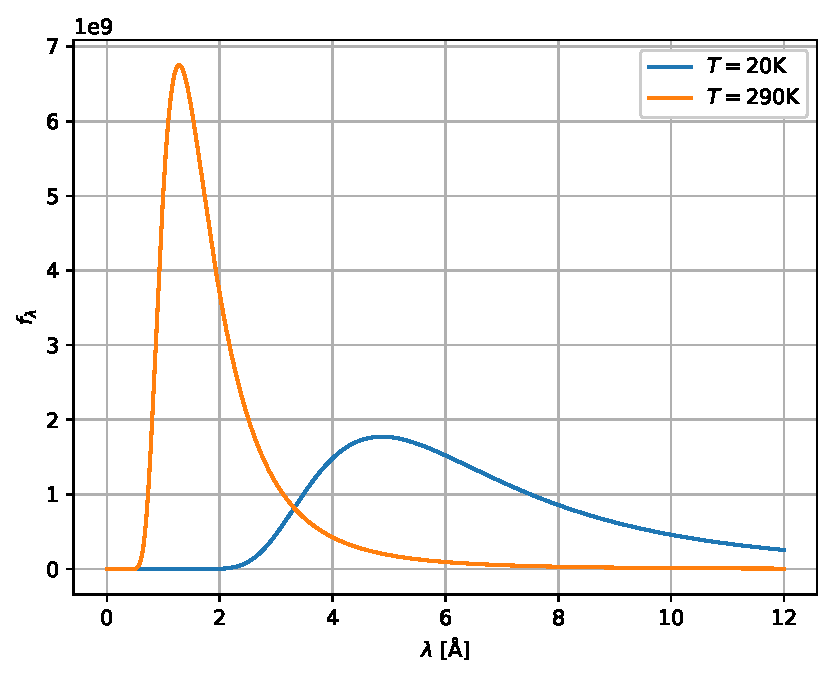
\includegraphics[width=0.5\linewidth]{source-spectrum}
	\caption{Probability density function for Maxwell-Boltzmann neutron sources at $T = 20 \unit{\kelvin}$ and $T = 290 \unit{\kelvin}$, illustrating the effect of using a cold neutron source.}
	\label{fig:source-spectrum}
\end{figure}

\subsection{Precession device analysis}
As discussed in Chapter \ref{c2:theory}, different precession devices can be derived that give a precession angle of the form of Equation \eqref{eq:precession-freq} resulting in modulation. The three main types existent in literature are isosceles triangles \cite{sales2015}, magnetic Wollaston prisms \cite{li2021} and ferromagnetic foil flippers \cite{bouwman2021b} and all three have previously been used in SEMSANS realizations and simulations. Their respective geometries are shown in Figure \ref{fig:precession-devices}. What they all have in common is that their effect is proportional to $\cot(\theta)$ and magnetic field strength $B$.
\subsubsection{Isosceles triangles}
In the case of a triangle as illustrated in Figure \ref{fig:precession-devices:iso}, the angle of the faces with the $z$-axis can be seen to be $\theta_0 = \arctan\left(\frac{h}{d/2}\right)$. Consider the triangle to be centred along the optical axis so that $y=0$ bisects it. Then for a path at height $y$, the length $L$ passed through the field becomes
$$L = d/2 - \frac{2y}{\tan\theta_0}$$
Using the Equation \eqref{eq:larmor-prec}, the precession angle after passing through the triangle becomes
$$\phi = c\lambda B L = c\lambda B(d/2 - \frac{2y}{\tan\theta_0})$$
Next, consider two similar triangles with base $d_1, d_2$ and field strengths $B_1, B_2$. Adding their precession angles gives 
$$\phi = c\lambda (B_1d_1/2 +B_2d_2/2) - 2c\lambda (B_1 + B_2) \frac{y}{\tan\theta_0}$$
To achieve $\phi = 0$ at $y=0$, the condition $B_1d_1 = -B_2d_2$ must hold, giving 
$$\phi = -2c\lambda (B_1 + B_2) \frac{y}{\tan\theta_0}$$
This can be achieved by making the triangle with the stronger field the smallest. 

\subsubsection{Magnetic Wollaston prisms}
A more sophisticated device is the magnetic Wollaston prism shown in Figure \ref{fig:precession-devices:wsp}, having two equal and opposite triangular magnetic fields in the form of a square. The analysis is very similar to that of isosceles triangles and for a single prism with angle $\theta_0$, the precession angle is
$$\phi = \frac{2c\lambda B y}{\tan{\theta_0}}$$
Two prisms with fields $B_1, B_2$ in sequence gives
$$\phi = \frac{2c\lambda (B_1 + B_2) y}{\tan{\theta_0}}$$
\subsubsection{Ferromagnetic foil flippers}
The last device type considered is the ferromagnetic foil flipper depicted in Figure \ref{fig:precession-devices:foil}. It consists of a ferromagnetic foil of thickness $d = 3\unit{\micro\meter}$ in an electromagnet which quickly saturates to a magnetization of $B_s = 1.0 \unit{\tesla}$ \cite{kraan2003}. The foil has the effect of rotating neutron spins around it by an angle 
$$\phi_{foil} = \frac{cdB_s\lambda}{\sin\theta_0}$$
By appropriately choosing $\theta_0$, the foil can be made to rotate a central wavelength $\lambda_0$ by $\phi_{foil} = \pi$, causing the device to emulate a magnetic Wollaston prism using a simpler magnetic field as the effect of the second triangular region behind the foil will be opposite to that of the first for $\lambda = \lambda_0$. In this case,
$$\phi = -2c\lambda (B_1 + B_2) \frac{y}{\tan\theta_0}$$
For $\lambda \neq \lambda_0$ this will cause a depolarization as was previously shown experimentally \cite{kraan2003}.
% I think because there is then a y-component of spin which shows up as 50/50 up/down on the detector. 
\begin{figure}[htbp]
	\centering
	\begin{subfigure}[b]{0.3\textwidth}
		\centering
		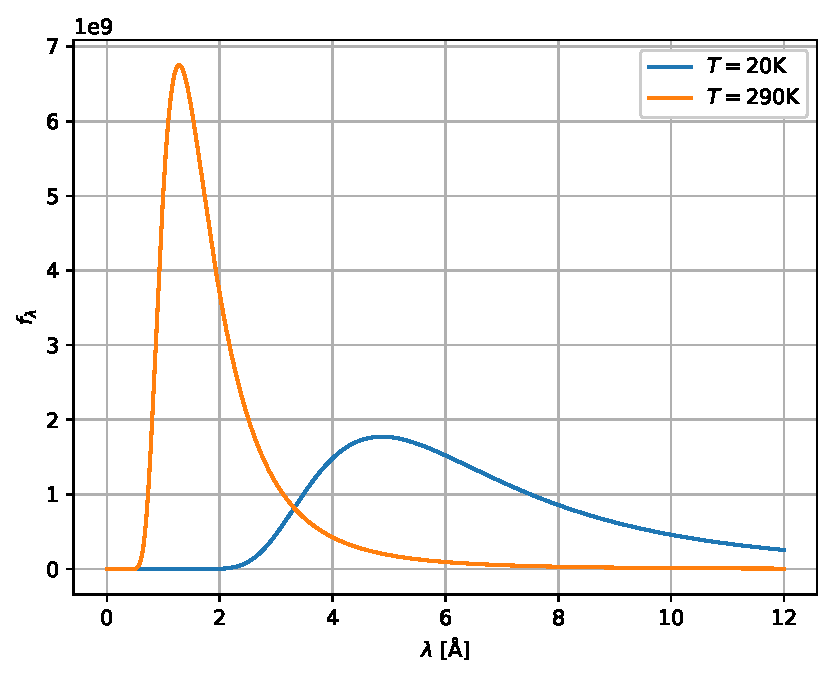
\includegraphics[width=\textwidth]{source-spectrum}
		\caption{CAPTION FOR ISO}
		\label{fig:precession-devices:iso}
	\end{subfigure}
	\hfill
	\begin{subfigure}[b]{0.3\textwidth}
		\centering
		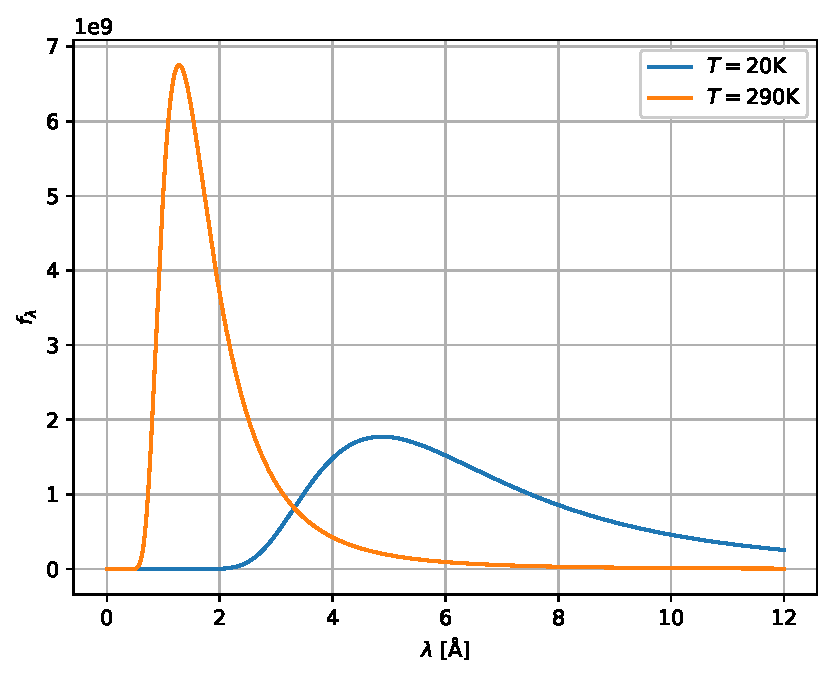
\includegraphics[width=\textwidth]{source-spectrum}
		\caption{CAPTION FOR WSP}
		\label{fig:precession-devices:wsp}
	\end{subfigure}
	\hfill
	\begin{subfigure}[b]{0.3\textwidth}
		\centering
		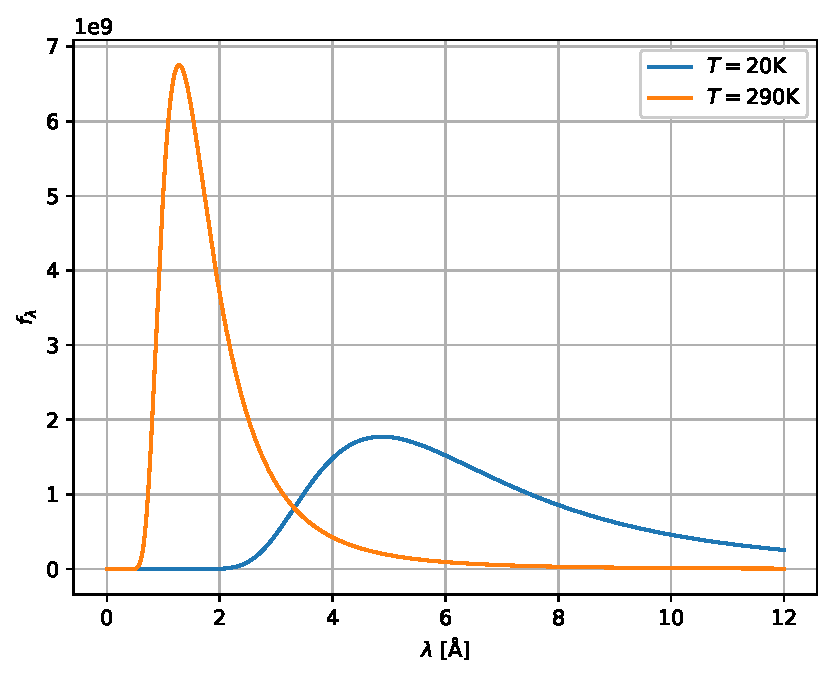
\includegraphics[width=\textwidth]{source-spectrum}
		\caption{CAPTION FOR FOIL}
		\label{fig:precession-devices:foil}
	\end{subfigure}
	\caption{TODO: THIS SHOULD CONTAIN 3 SUBFIGURES SHOWCASING THE DEVICE GEOMETRIES NEXT TO EACH OTHER TO FACILITATE COMPARISON}
	\label{fig:precession-devices}
\end{figure}

\subsubsection{Device $\alpha$ and characteristics}
In summary, once device-specific conditions are met a pair of any of them have in absolute terms the same precession-angle profile given by Equation \eqref{eq:precession-freq} with $\alpha = \frac{(B_1 + B_2)}{\pi\tan\theta_0}$
\begin{equation}
	\phi = 2c\lambda (B_1 + B_2)\frac{y}{\tan\theta_0} \label{eq:device-prec}
\end{equation}
the contribution of each separate device being $\phi_i = \frac{2c\lambda B_i y}{\tan\theta_0}$. Table \ref{tab:device-properties} summarizes device characteristics as they appear in literature that will be used in this research.

\begin{table}[h!]
	\centering
	\begin{tabular}{|c|c|c|c|c|c|}
		\hline
		Name & Label & $\theta_0$ (degrees) & $B_{\text{min}}$ (mT) & $B_{\text{max}}$ (mT) & Source \\
		\hline
		Isosceles triangle & ISO & 20 & 0.1 & 15 & \cite{kusmin2017} \\
		Wollaston prism & WSP & 45 & 0.1 & 63 & \cite{li2021} \\
		Foil flipper & FOIL & - & 0.3 & 30 & \cite{bouwman2011} \\
		\hline
	\end{tabular}
	\caption{Precession device characteristics including the source of the values used. For a foil flipper, $\theta_0$ needs to be set to match $\lambda_0$ and is omitted, its range is sufficient for all $\lambda_0$'s considered in this research.}
	\label{tab:device-properties}
\end{table}
\subsubsection{Focussing condition}
In practice, neutrons will not travel parallel to the $z$-axis but move at a slight angle to this depending on beam divergence and other parameters. Letting $\theta$ be the angle their trajectory makes with the $z$-axis in the $yz$ plane, it can be seen that a neutron arriving at height $y$ on the detector will pass through the $i$'th precession device at average height $y_i = y + L_i\tan\theta \approx y + L_i\theta$, with $L_i$ being the distance from the detector of the device. This means that the total precession angle will be
$$\phi = 2c\lambda B_1\frac{y + L_1\theta}{\tan\theta_0} + 2c\lambda B_2\frac{y + L_2\theta}{\tan\theta_0}$$
This $\theta$-dependence is a problem as it will cause a loss of modulation depending on how large $\theta$ is. In first-order approximation, this effect can be removed by setting the positions $L_i$ and field strengths $B_i$ to meet the focussing condition
$$B_1L_1 = -B_2L_2$$
Substituting this retrieves Equation \eqref{eq:device-prec}. This gives also the motivation for using two devices: you need at least two to remove this $\theta$-dependency and achieve optimal modulation using a realistic, slightly divergent beam.
\subsection{Detector characteristics}
The position sensitive detector used is $11\times11\unit{\milli\meter}$ with a resolution of $1001$ pixels along the $y$-axis, corresponding to a pixel size of approximately $p = 10\unit{\micro\meter}$ with detector height $h_d = 11\unit{\milli\meter}$. It is assumed that the neutron beam size and divergence is such that the full detector is used (TODO: EXPAND DISCUSSION OF BEAM SIZE, DIVERGENCE, ACCEPTANCE ANGLES?). As will be discussed in detail in Chapter \ref{c4:constraints}, the detector size and resolution in this case limits modulation frequencies $f = \alpha\lambda$ that can be sampled.

\subsection{Polychromatic SEMSANS}
The usual description of SEMSANS modulation patterns as given in \eqref{eq:mono-modulation} and their relation to a spin-echo length \eqref{eq:delta} typically assumes a monochromatic source or a source that closely approximates it, for instance by using a PG monochromator with $\Delta\lambda/\lambda_0 = 0.01$ with thermal neutrons. However, even in such cases a modulation envelope can be seen to appear \cite{bouwman2021} due to this wavelength spread. This effect becomes far more important when using a velocity selector with $\Delta\lambda/\lambda_0 = 0.1$ to select a higher wavelength $\lambda_0$ and is here discussed in detail.
%Without resorting to time-of-flight instrument realizations also exist \cite{sales2015}\cite{li2021} that in this way support broad ranges of wavelengths. 
\subsubsection{Modulation envelope for Gaussian $\lambda$ spectrum}
Assuming a Gaussian wavelength distribution as given by Equation \eqref{eq:gauss-spectrum} and neglecting wavelength-specific effects like foil flipper polarization loss, it can be shown using Fourier analysis that the base intensity modulation becomes
\begin{equation}
	I_b(y) = I_{0,b} + A_bE(y)\cos(2\pi\alpha\lambda_0y) \label{eq:poly-base-modulation}
\end{equation}
The envelope $E(y)$ is a Gaussian and given by
\begin{equation}
	E(y) = e^{-\frac{1}{2}\left(2\pi\alpha\sigma y\right)^2} \label{eq:poly-base-modulation-env}
\end{equation}
Substituting $\sigma=0$ for a monochromatic limit gives back Equation \eqref{eq:mono-modulation}. This modulation envelope $E(y)$ can be shown to have FWHM 
\begin{equation}
	FWHM_E = \frac{\sqrt{2\ln 2}}{\pi\alpha\sigma} \label{eq:poly-base-modulation-fwhm}
\end{equation}
From this it can clearly be seen that increasing wavelength spread $\sigma$ results in a narrower modulation envelope width. It also confirms the envelope narrowing observed when increasing $B$ field strengths (proportional to $\alpha$) \cite{bouwman2021}. 
\subsubsection{Effect on interaction with sample and $\delta$-resolution}
At first glance, it is clear that the effect of a sample on the modulation will be more complicated than a simple reduction of the amplitude of the modulation envelope. The modulation now consists of a range of wavelengths $\lambda$, each related to a spin-echo length $\delta = \lambda^2 L_s\alpha$ and each with a scattering power $\tau \propto\lambda^2$ such as Equation \eqref{eq:sample-tau}. Although Equations \eqref{eq:mono-modulation} and \eqref{eq:sample-pol-reduction} by itself do not describe the corresponding modulation pattern, they do describe what happens to a single frequency so that
\begin{equation}
	I_s(y) = I_{0,s} + \int_{-\infty}^\infty f_{\text{gauss}}(\lambda)e^{G(\lambda^2 L_s\alpha) - \tau(\lambda)}A_b\cos(2\pi\alpha\lambda y)d\lambda \label{eq:poly-sample-modulation}
\end{equation}
per linearity describes the modulation pattern. Qualitatively it can be seen that for greater $\sigma$, a greater $\delta$ range is accessed around a central value corresponding to $\lambda_0$ and reflected in the spectrum. This means that estimating $G(\delta)$ from the visibility will introduce error depending on the specific sample and the $\delta$-resolution will be limited. One way to avoid this problem is to compute the Fourier spectrum and consider the transfer of the sample in the frequency domain. This does bring with it new problems such as frequency resolution limitations. 


\subsection{Instrument design variants}
Using the basic instrument configuration described and analysed in this chapter with the various options in terms of monochromator and precession devices, a few design variants can be formulated exploring the different options. What they have in common are the distances in the instrument $L_1 = 4.0\unit{\meter}, L_2 = 2.0\unit{\meter}, L_s = 1.8\unit{\meter}$ in addition to the detector characteristics previously described. The possibility of optimizing these distances together with $\lambda_0$ for a given choice of monochromator and precession device is discussed in Chapter \ref{c5:optimization}.  

Firstly, there is the choice of $\lambda_0$ and the corresponding monochromator. Two considered options are $\lambda_0 = 4.321$Å with a PG monochromator giving $\Delta\lambda = 0.04321$Å and $\lambda_0 = 8$Å with a VS monochromator giving $\lambda_0 = 0.8$Å. These two sources are combined with each of the three precession device options as characterized in Table \ref{tab:device-properties}, giving Table \ref{tab:design-variants} which includes the appropriate $\theta_0$ needed to achieve $\phi_{foil} = \pi$ in the case of foil flippers. These instruments will first be analysed in the next chapter to estimate their $\delta$-range by using constraints as well as their relative source intensity. In Chapter \ref{c6:monte-carlo}, Monte Carlo simulation results of these instruments on a three representative samples are discussed. 

\begin{table}[h!]
	\centering
	\begin{tabular}{|c|c|c|c|c|c|c|c|}
		\hline
		Label & $\lambda_0$ (Å) & $\Delta\lambda$ (Å) & Monochromator & Device & $\theta_0$ (degrees) & $B_{\text{min}}$ (mT) & $B_{\text{max}}$ (mT) \\
		\hline
		ISO 4 & 4.321 & 0.04321 & PG & ISO & 20 & 0.1 & 15 \\
		WSP 4 & 4.321 & 0.04321 & PG & WSP & 45 & 0.1 & 63 \\
		FOIL 4 & 4.321 & 0.04321 & PG & FOIL & 11.0138 & 0.3 & 30 \\
		ISO 8 & 8 & 0.8 & VS & ISO & 20 & 0.1 & 15 \\
		WSP 8 & 8 & 0.8 & VS & WSP & 45 & 0.1 & 63 \\
		FOIL 8 & 8 & 0.8 & VS & FOIL & 20.71416 & 0.3 & 30 \\
		\hline
	\end{tabular}
	\caption{Various instrument design variants combining different $\lambda_0$ and monochromator pairings with the various precession device options. Designs are labelled by combining their device type and the (rounded) value of $\lambda_0$.}
	\label{tab:design-variants}
\end{table}

% $\psi_0 = 1^\circ$ or $\psi_0 = 0.01745329$ in radians



%\section{SEMSANS instrument model}
%In this chapter, the used SEMSANS instrument model and all its components with their basic functions as well as parameters is introduced. It is based on an instrument which was previously simulated (CITATION NEEDED) and which is available as NAME in the McStas instrument library. A schematic overview is given in ADD FIGURE HERE. 
%\subsection{Source}

%\section{Source}
% Key challenge: translate this beautiful blob of mathematics and analysis I have in my jupyter notebook to on the one hand a summary and theoretical background and on the other hand a (somewhat, at least in the extent of having fully worked it out myself generally unaware of existing derivations) novel analysis on which
% Another challenge: how to deal with the rather expansive theory with at least 2 main branches which there appears to be? If I give a theoretical background to make this thing readable for other bachelor students then I do sort of have to start at Larmor precession and neutron spins but also at small angle scattering and this is confusing. 

\newpage
\section{$\delta$-constraints and intensity in instrument design}
\label{c4:constraints}

\subsection{Constraints}
% Discuss sources of constraints, linking them to the theory in previous chapters. Ideally refer to equation numbers to avoid repetition and make it sound really solid. 
% Emphasize that these constraints serve as a starting point for estimating limitations for given instruments


\subsection{Coarse intensity estimate}
In addition to the $\delta$-range, the intensity is a key factor in instrument design: it determines the measurement time and quality in an experimental setting. Although accurate intensity estimates are beyond the scope of this research, requiring detailed characterizations of losses in all components and accounting for many factors, a highly simplified estimate assuming ideal components can be derived as follows.

First of all, the flux after the monochromator combined is estimated relative to the full-spectrum flux $\Phi_0 = 10^9 \unit{\centi\meter^{-2}\sec^{-1}}$ (TODO: change/add source). Given an operating point $\lambda_0$ with a matching $\sigma$ from the monochromator type, the intensity can be estimated by numerical evaluation of the integral
$$\Phi_{mc} \propto \Phi_0\int_0^\infty f_{\text{gauss}}(\lambda)e^{-\frac{1}{2}\left(\frac{\lambda - \lambda_0}{\sigma}\right)^2}d\lambda$$
The transfer of the monochromator is assumed to be a lossless Gaussian, and losses from beam divergence from beamline to monochromator are neglected.  It can easily be seen from Figure \ref{fig:source-spectrum} that the choice of $\lambda_0$ matters here, as well as the value of $\sigma$. Assuming an ideal polariser and an ideal analyser, the average loss of intensity for $\pm x$ analyser settings due to these corresponds to a factor $1/4$. To account for losses due to beam divergence, consider the beam divergence to be a small angle $\psi_0$. For a beam of radius $R_0$ at the end of the beamline, at a distance $d$ from the beamline, taken to be after the analyser, it will have expanded to radius $R = R_0 + \psi_0 d$ in small-angle approximation. Simplifying the distribution of neutrons to be uniform over this expanded radius, the flux at distance $d$ can be seen to be proportional to
$$\Phi(d) \propto \frac{\Phi_{mc}}{4}\frac{R_0^2}{(R_0 + \psi_0 d)^2}$$
This expression can be used to compute a very coarse estimate for an upper bound of the total sample or detector intensity by substituting the respective distances $d$ from the source and integrating the flux over the surface area.   

\subsection{Limitations of constraint scheme}
% Discuss things that are missing
% Also very important: discuss the softer constraints: why should the envelope FWHM be 3mm and not 2mm or 4mm? What determines this other than vibes. Indicate how they could be made more/less flexible

\subsection{Computed $\delta$ constraints and final design $\delta$ ranges}
% Give a table of computed constraints per instrument with ideally great names



\subsection{Discussion of designs}
% Here I'll write about clear trends in the tables of limitations and give indications of what is limiting these instruments. It might be interesting to give concrete recommendations: in order to get an even better delta range you could get a different monochromator, boost the B fields etc.

\newpage
\section{Optimization of instrument parameters}
\label{c5:optimization}
TODO: FINISH THIS CHAPTER, ADDING OPTIMAL INSTRUMENT DESIGNS AND PERFORMANCE.
%The problem of designing an instrument suitable for a specific length range like \targetrange subject to the various constraints indicated in the previous chapter can be aptly described as a constrained optimization problem. This does require a formulation of an objective function to maximize and generally speaking this is easier said than done if all factors including instrument cost, intensity etc. are to be taken into account in addition to the $\delta$-range. In this section, the function that is maximized only depends on the $\delta$-range and consequently it should be understood as a speculative exploration of the instrument parameter-space rather than a final optimization of instruments to realize. At best, the presented optimal instruments represent the best one can do in terms of $\delta$-range in the framework of parameters and constraints considered in this research.

\subsection{Two possible $\delta$-range objective functions}
Given the constraints formulated in Chapter \ref{c4:constraints}, let $(\delta_{i, min},\delta_{i, max})$ be the final $\delta$ interval subject to these constraints and let $(\delta_{t, min},\delta_{t, max})$ be a target interval. If these overlap, let the overlap interval be given by $(\delta_{o, min},\delta_{o, max})$. A first objective function $g_1$ to maximize is ratio of the length of the overlap and the length of the target interval
$$g_1 = \begin{cases}
	\frac{\delta_{o, max}-\delta_{o, min}}{\delta_{t, max} - \delta_{t, min}},\text{ if $\delta$-ranges overlap}\\
	0,\text{ else}
\end{cases}$$
A problem with this objective function is that it doesn't take into consideration that the instrument should perform well across different length ranges and is biased towards the higher $\delta$ values in optimal designs. An intuitive way to optimize for coverage of different length ranges is achieved by looking at these on a logarithmic scale and considering the overlap there, which can be expressed using a second objective function $g_2$ as follows 
$$g_2 = \begin{cases}
	\frac{\ln(\delta_{o, max}/\delta_{o, min})}{\ln(\delta_{t, max}/\delta_{t, min})},\text{ if $\delta$-ranges overlap}\\
	0,\text{ else}
\end{cases}$$

\subsection{Optimization scheme}
Similar to in the previous chapter, all different pairings of precession devices and monochromators are considered. However, $\lambda_0, L_1, L_2, L_s$ are now free parameters with $\lambda_0$ being bounded by the approximate $\lambda$-band of the respective monochromator. 

\subsection{Discussion of optimal instruments}
% The resulting optimal instrument parametrizations confirm patterns already visible in the previous chapter. For instance, isosceles triangles seem to be a very bad pairing with a PG monochromator. It can also be seen that instruments with PG monochromators are generally bounded on the upper end by field strength and those with velocity selectors by the narrowing of their envelope caused by wavelength spread. Similarly, almost all instruments are bounded by the condition that at least one period must be visible on the detector, with especially instruments at greater wavelengths $\lambda_0$ suffering from this limitation.  
% add further points that come up, maybe after writing a similar section for designs and their computed limitations
\newpage
\section{Monte Carlo simulations of designs using McStas}
\label{c6:monte-carlo}
% after all the analysis and discussion of constraints/optimizing using these, introduce monte carlo simulations as a step closer to a practical instruments and a way to verify identified limitations and see them in play. This last aspect could be an interesting part of the discussion of simulation results as well, you can really point out narrowing modulation envelopes, modulation periods becoming too big for the detecto retcetera. 
% I expect some designs to not be able to measure specific samples at all or barely to the extent that showing them in a plot is a bit silly. 

\subsection{Simulation setup}
% Mention the three samples, perhaps discuss their properties like thickness t etc. besides R. You can just put them in a table quick and dirty.
% Maybe repeat/put an analytical graph of the expected P(\delta) curve here for all 3.
\subsection{Results}
% There will be quite a few graphs here, maybe use Appdendices if it is too much!
\subsection{Discussion}
% Did the simulations match the precomputed limits? Are the limits (to the extent that they are not absolute but rather somewhat chosen heuristically) good enough, too strict? Is it in practice possible to measure even at field strenghts outside of the range?

%\section{Appendix A: Limitations of SEMSANS theory at lower end of $\delta$ range}
%In elastic scattering, the initial and final wave vectors $k_i$, $k_f$ are related through wave vector transfer $Q = |k_f - k_i| = k 2\sin\theta$ with $2\theta$ being the angle between $k_i, k_f$ and $|k_i| = |k_f| = k$ due to elasticity. 

%In normal SEMSANS theory, the small-angle approximation must hold so that $Q_y = k2\theta$ or with $2\theta %\approx \frac{y}{L_s}$, $Q_y = k\frac{y}{L_s}$. Using this approximation, it can be seen that $\phi_t = %\delta Q_y$, which means that the modulation amplitude $A(\delta)$ is related to
%$$G(\delta) = \frac{1}{\sigma k^2}\int_{Q_{x,min}}^{Q_{x,max}}\int_{Q_{y,min}}^{Q_{y,max}}\dfrac{d\sigma}{d\Omega}(Q)cos(\delta Q_y)dQ_ydQ_x$$
%by the formula
%$$A(\delta) = e^{\sigma [G(\delta) - 1]}$$
%It can be shown that the generally correct expression for $Q_y$ is 
%$$Q_y = 2k\sin(\frac{\arctan\frac{y}{L_s}}{2})$$
%This can be simplified to the somewhat lengthy expression
%$$Q_y = 2k \frac{\frac{y}{L_s}}{\sqrt{2}\sqrt{\frac{y^2}{L_s^2} + 1 }\sqrt{\frac{1}{\sqrt{\frac{y^2}{L_s^2} + 1}}+1}}$$
%Considering again small $\frac{y}{L_s}$, it can be derived using a Taylor expansion that
%$$Q_y \approx  k(\frac{y}{L_s} - \frac{3y^3}{8L_s^3})$$
%So a more accurate relation between $\phi_t$ and $Q, \delta_y$ is given by $$\phi_t = \frac{\delta Q_y}{1 - \frac{3y^2}{8L_s^2}}$$
% This appears to give an indication of up to which angles the SEMSANS theory gives a correct description of the amplitude decrease.
\newpage
\section{Conclusion and future work}




\printbibliography
\end{document}
